\title{Assignment 8}
\author{
        Avijit Ghosh \\
        14CH3FP18\\
}
\date{\today}

\documentclass[12pt]{article}
\usepackage{graphicx}
\usepackage[utf8]{inputenc}
\usepackage{times}


\begin{document}
\maketitle

\begin{abstract}
Event-driven Simulation of random particle collisions using heaps.
\end{abstract}

\section{Introduction}
This program simulates the collision of balls on a 2D planar region bounded by straight walls using a Heap Data Structure.\\

\section{Event Driven Simulation}
We need to devise the most efficient use of the Heap data structure to simulate the collision of particles using Event driven simulation. \\
Event driven simulation allows us to simulate events in a chronological order.\\

\section{Implementation}\label{Implementation}
The implementation of the is described as below:\\
\paragraph{Particle}
The particle structure describes a sphere. It has a radius, initial x, y coordinates and initial vx, vy velocity values. Each particle also has a color. All these are randomly assigned.\\

\paragraph{List}
Each particle also has a linked list attached to the particle. The linked list keeps track of all the valid collisions that the particular particle has participated in. This list is later purged to obtain the data for our plot.\\

\paragraph{Collision Heap}
The Heap structure is what maintains the entire event data for the system. Using equations of motion we predict the next event and insert it into the heap. The heap is a min-heap, which means that the earliest event is at the top.\\
The heap is implemented as a very large array, with data members being Particle A and B (the two particles that take part in collision). In case the collision is with a wall, one of them is null. \\
The main loop runs until the heap is empty and the prediction function is called until the logical time is greater than or equal to the intended time of simulation.\\

\paragraph{Validity Check}
The validity of a collision event is checked as follows:\\


			\textbf{isValid(CollisionHeap A)} \\
			\indent \indent if (A.a != NULL and count(A.a) != A.countA)\\ 
			\indent \indent \indent return false;\\
			\indent \indent if (A.b != NULL and count(A.b) != A.countB)\\ 
			\indent \indent \indent return false;\\
			\indent \indent return true;\\
		




\paragraph{Insertion}
Pseudocode for insertion of events: \\ \\
\textbf{void Insert(CollisionHeap H[], CollisionHeap Element)}\\

	\indent \indent i=0;\\
	\indent \indent heapsize++;\\
	\indent \indent H[heapsize]$\leftarrow$Element;\\
   \indent \indent now$\leftarrow$heapsize;\\
   \indent \indent while(H[now/2].timestamp $\textgreater$ Element.timestamp)\\
   \indent \indent\indent H[now]$\leftarrow$H[now/2];\\
   \indent \indent\indent now/=2;\\
   \indent \indent H[now]$\leftarrow$Element;\\
\\

\paragraph{Minimum Element extraction and Deletion}
Pseudocode for extracting the next event and deleting it from the Heap:\\ \\

\textbf{CollisionHeap NextDelete(CollisionHeap H[])}\\

        \indent CollisionHeap minElement,lastElement;\\
        \indent int child,now;\\
        \indent minElement $\leftarrow$ H[1];\\
        \indent lastElement $\leftarrow$ H[Heapsize--];\\

        \indent for(now = 1; now*2 $\textless$= Heapsize ;now = child)\\
                \indent\indent child $\leftarrow$ now*2;\\          
                \indent\indent if(child not equals Heapsize and H[child+1].timestamp $\textless$ H[child].timestamp ) \\
                        \indent\indent\indent child++;\\
                \indent\indent if(lastElement.timestamp $\textgreater$ H[child].timestamp)\\
                        \indent\indent\indent H[now] $\leftarrow$ H[child];\\
                \indent\indent else\\
                        \indent\indent\indent break;\\
        \indent H[now] $\leftarrow$ lastElement;\\
        \indent return minElement;\\
\\

\subsection{Complexity Analysis}\label{Complexity Analysis}
\paragraph{Insertion}
Insertion requires adding an event to its specific linked list followed by updating the heap upwards from the linked list towards the root. This operation consumes $\theta(log(n))$ number of operations, where $\mathbf{n}$ is the number of particles in the system.
 
\paragraph{Extraction of minimum and deletion}
The minimum element is at the top due to the heap property, so obtaining it takes $\theta(1)$ time.\\
Now we take the max element and put it at the top, then recursively swap it with its children until the heap property is restored.\\
In the worst case, the new root has to be swapped with its child on each level until it reaches the bottom level of the heap, meaning that the delete operation has a time complexity relative to the height of the tree, or $\theta(log(n))$\\\


\section{Plots}\label{plots}


\begin{figure}[ht!]
\centering
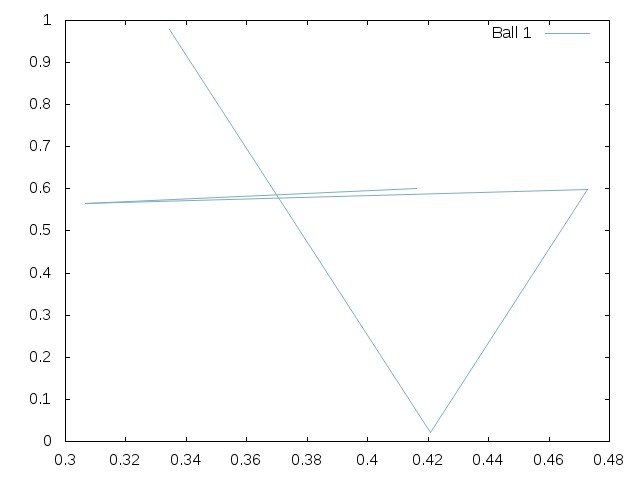
\includegraphics[width=12cm]{plot1.jpg}
\end{figure}

\begin{figure}[ht!]
\centering
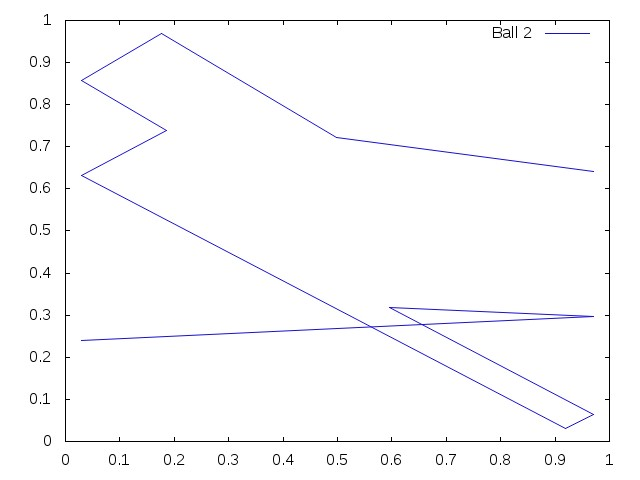
\includegraphics[width=12cm]{plot2.jpg}
\end{figure}

\begin{figure}[ht!]
\centering
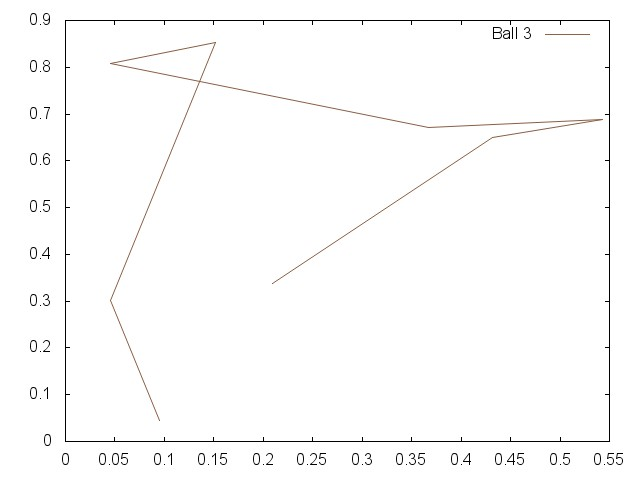
\includegraphics[width=12cm]{plot3.jpg}
\end{figure}

\begin{figure}[ht!]
\centering
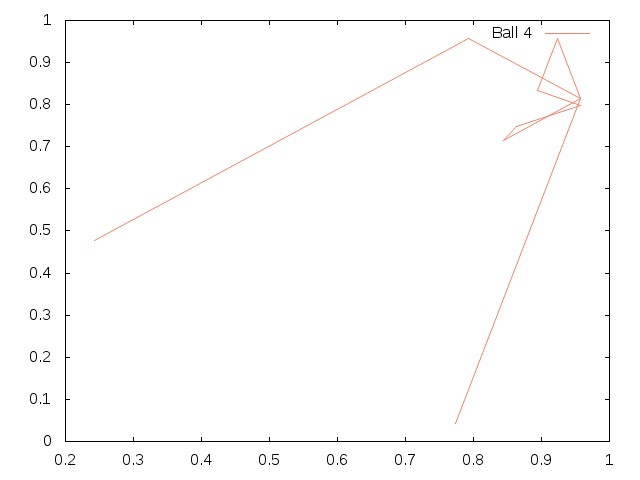
\includegraphics[width=12cm]{plot4.jpg}
\end{figure}

\begin{figure}[ht!]
\centering
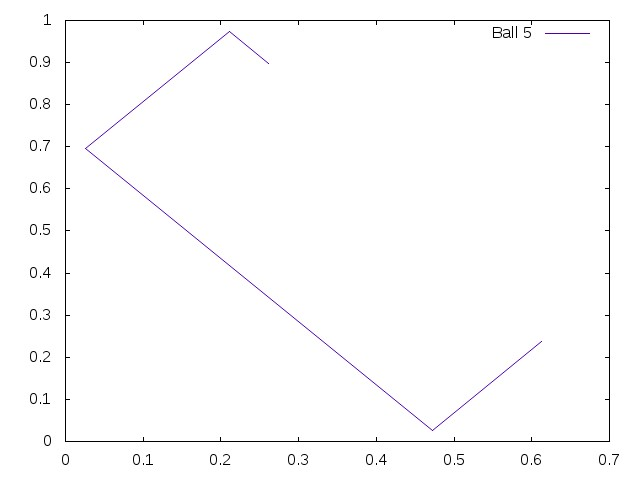
\includegraphics[width=12cm]{plot5.jpg}
\end{figure}

\end{document}